\input{../utils/preamble}
\createdgmtitle{7}
%--------------------------------------------------------------------------------
\begin{document}
%--------------------------------------------------------------------------------
\begin{frame}
%\thispagestyle{empty}
\titlepage
\end{frame}
%=======
\begin{frame}{Dequantization}
	\begin{itemize}
		\item Images are discrete data, pixels lie in the [0, 255] integer domain (the model is $P(\bx | \btheta) = \text{Categorical}(\bpi(\btheta))$).
		\item Flow is a continuous model (it works with continuous data $\bx$).
	\end{itemize}
	By fitting a continuous density model to discrete data, one can produce a degenerate solution with all probability mass on discrete values. \\
	How to convert a discrete data distribution to a continuous one?
	
	\begin{minipage}[t]{0.5\columnwidth}
		\begin{block}{Uniform dequantization}
		\vspace{-0.5cm}
			\begin{align*}
				\bx &\sim \text{Categorical}(\bpi) \\
				 \bu &\sim U[0, 1]
			\end{align*}
			\[
			\by = \bx + \bu \sim \text{Continuous} 
			\]
		\end{block}
	\end{minipage}%
	\begin{minipage}[t]{0.5\columnwidth}
		\begin{figure}
			\centering
			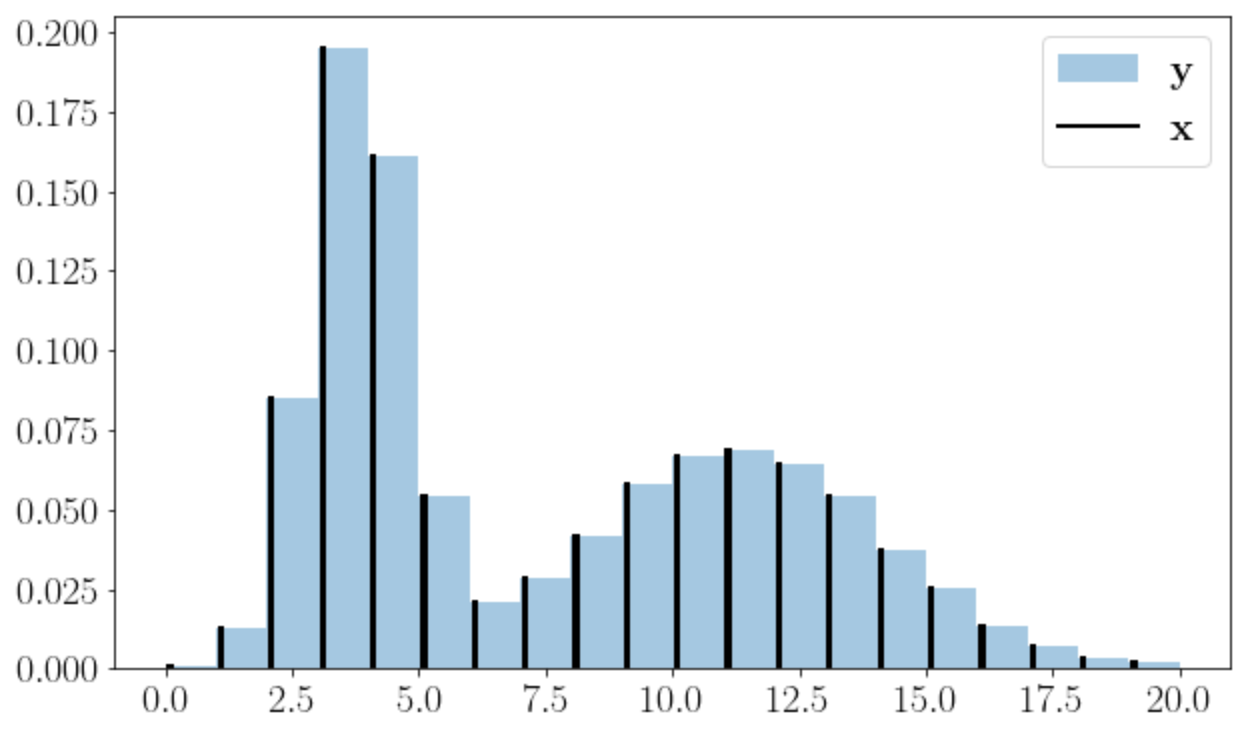
\includegraphics[width=1.0\linewidth]{figs/uniform_dequantization.png}
		\end{figure}
	\end{minipage}
	\myfootnotewithlink{https://arxiv.org/abs/1511.01844}{Theis L., Oord A., Bethge M. A note on the evaluation of generative models. 2015}
\end{frame}
%=======
\begin{frame}{Uniform dequantization}
	\begin{block}{Statement}
		Fitting continuous model $p(\by | \btheta)$ on uniformly dequantized data $\by = \bx + \bu, \, \bu \sim U[0, 1]$ is equivalent to maximization of a lower bound on log-likelihood for a discrete model:
		\[
		P(\bx | \btheta) = \int_{U[0, 1]} p(\bx + \bu | \btheta) d \bu
		\]
		\vspace{-0.2cm} \\
		Thus, the maximisation of continuous model log-likelihood on $\by$ can't lead to the a collapse onto the discrete data (the objective is bounded above by the discrete model log-likelihood).
	\end{block}
	\begin{block}{Proof}
		\vspace{-1cm}
		\begin{multline*}
			 \log P(\bx | \btheta) = \log \int_{U[0, 1]} p(\bx + \bu | \btheta) d \bu \geq \\ \geq \int_{U[0, 1]} \log p(\bx + \bu | \btheta) d \bu = \log p(\by | \btheta).
		\end{multline*}
	\end{block}
\end{frame}
%=======
\begin{frame}{Variational dequantization}
	\begin{minipage}[t]{0.5\columnwidth}
			\begin{figure}
				\centering
				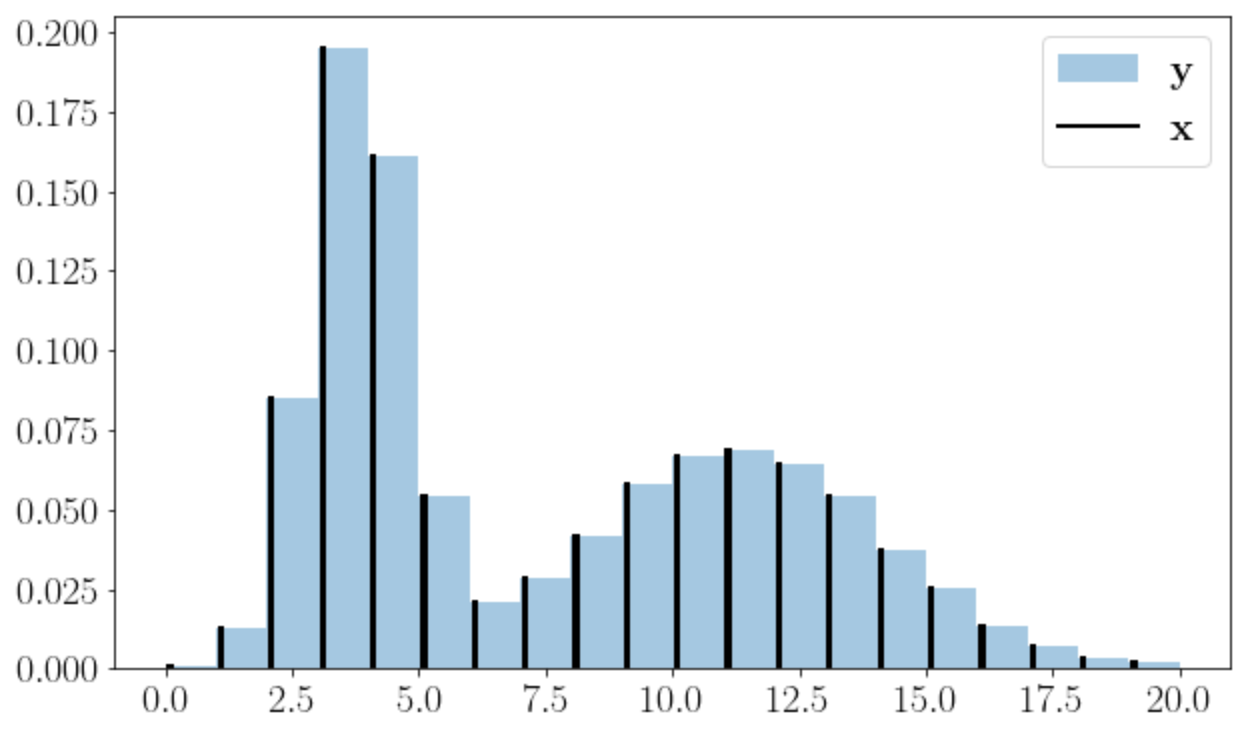
\includegraphics[width=1.0\linewidth]{figs/uniform_dequantization.png}
			\end{figure}
	\end{minipage}%
	\begin{minipage}[t]{0.5\columnwidth}
		\begin{figure}
			\centering
			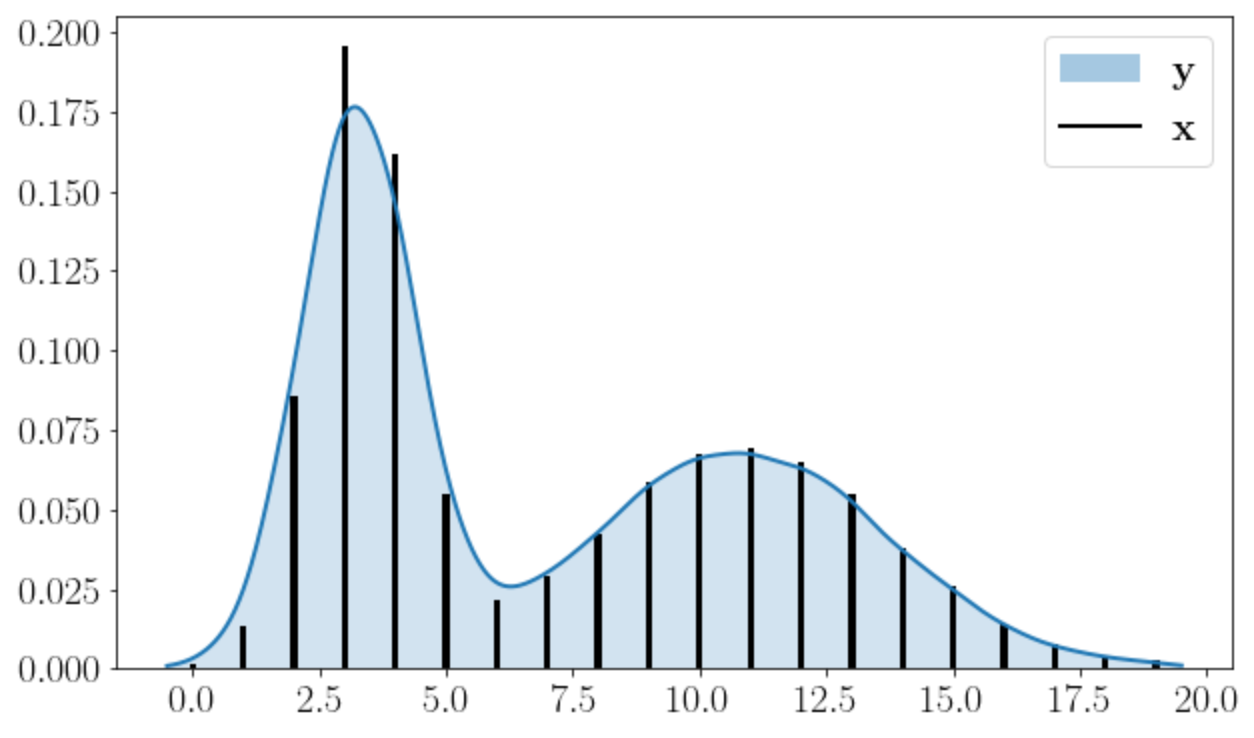
\includegraphics[width=1.0\linewidth]{figs/variational_dequantization.png}
		\end{figure}
	\end{minipage}
	\begin{itemize}
		\item $p(\by | \btheta)$ assign unifrom density to unit hypercubes $\bx + U[0, 1]$ (left fig).
		\item Neural network density models are smooth function approximators (right fig).
		\item Smooth dequantization is more natural.
	\end{itemize}
	How to perform the smooth dequantization? \\
\end{frame}
%=======
\begin{frame}{Flow++}
	\begin{block}{Variational dequantization}
		Introduce variational dequantization noise distribution $q(\bu | \bx)$ and treat it as an approximate posterior. 
	\end{block}
	\begin{block}{Variational lower bound}
		\vspace{-0.7cm}
		\begin{multline*}
		 \log P(\bx | \btheta) = \left[ \log \int q(\bu | \bx) \frac{p(\bx + \bu | \btheta)}{q(\bu | \bx)} d \bu \right] \geq \\ 
			\geq  \int q(\bu | \bx) \log \frac{p(\bx + \bu | \btheta)}{q(\bu | \bx)} d \bu = \mathcal{L}(q, \btheta).
		\end{multline*}
	\end{block}
	\vspace{-0.5cm}
	\begin{block}{Uniform dequantization bound}
		\vspace{-0.7cm}
		\begin{multline*}
		 \log P(\bx | \btheta) = \log \int_{U[0, 1]} p(\bx + \bu | \btheta) d \bu \geq \\ \geq \int_{U[0, 1]} \log p(\bx + \bu | \btheta) d \bu = \log p(\by | \btheta).
		\end{multline*}
	\end{block}
	\myfootnotewithlink{https://arxiv.org/abs/1902.00275}{Ho J. et al. Flow++: Improving Flow-Based Generative Models with Variational Dequantization and Architecture Design, 2019}
\end{frame}
%=======
\begin{frame}{Flow++}
	\begin{block}{Variational lower bound}
		\[
		\mathcal{L}(q, \btheta) = \int q(\bu | \bx) \log \frac{p(\bx + \bu | \btheta)}{q(\bu | \bx)} d \bu.
		\]
	\end{block}
	Let $\bu = h(\bepsilon, \bphi)$ is a flow model with base distribution $\bepsilon \sim p(\bepsilon) = \mathcal{N}(0, \mathbf{I})$:
	\vspace{-0.3cm}
	\[
		q(\bu | \bx) = p(h^{-1}(\bu, \bphi)) \cdot \left| \det \frac{\partial h^{-1}(\bu, \bphi)}{\partial \bu}\right|.
	\]
	\vspace{-0.3cm}
	Then
	\[
		\log P(\bx | \btheta) \geq \cL(\bphi, \btheta) = \int p(\bepsilon) \log \left( \frac{p(\bx + h(\bepsilon, \bphi) | \btheta)}{p(\bepsilon) \cdot \left| \det \frac{\partial h(\bepsilon, \bphi)}{\partial \bepsilon}\right|^{-1}} \right) d\bepsilon.
	\]
	\myfootnotewithlink{https://arxiv.org/abs/1902.00275}{Ho J. et al. Flow++: Improving Flow-Based Generative Models with Variational Dequantization and Architecture Design, 2019}
\end{frame}
%=======
\begin{frame}{Flow++}
	\begin{block}{Variational lower}
	\vspace{-0.3cm}
	\[
		\log P(\bx | \btheta) \geq \int p(\bepsilon)\log \left( \frac{p(\bx + h(\bepsilon, \bphi))}{p(\bepsilon) \cdot \left| \det \frac{\partial h(\bepsilon, \bphi)}{\partial \bepsilon}\right|^{-1}} \right) d\bepsilon.
	\]
	\end{block}
	\begin{itemize}
	\item If $p(\bx + \bu | \btheta)$ is also a flow model, it is straightforward to calculate stochastic gradient of this ELBO.
	
	\item Uniform dequantization is a special case of variational dequantization ($q(\bu | \bx) = U[0, 1]$).
	The gap between $\log P(\bx | \btheta)$ and the derived ELBO is 
	$ KL(q(\bu | \bx) || p(\bu | \bx))$.
	\item In the case of uniform dequantization the model unnaturally places uniform density over each hypercube $\bx + U[0, 1]$ due to inexpressive distribution $q$.
	\end{itemize}
	\myfootnotewithlink{https://arxiv.org/abs/1902.00275}{Ho J. et al. Flow++: Improving Flow-Based Generative Models with Variational Dequantization and Architecture Design, 2019}
\end{frame}
%=======
\begin{frame}{Flow++}
	\begin{figure}
		\centering
		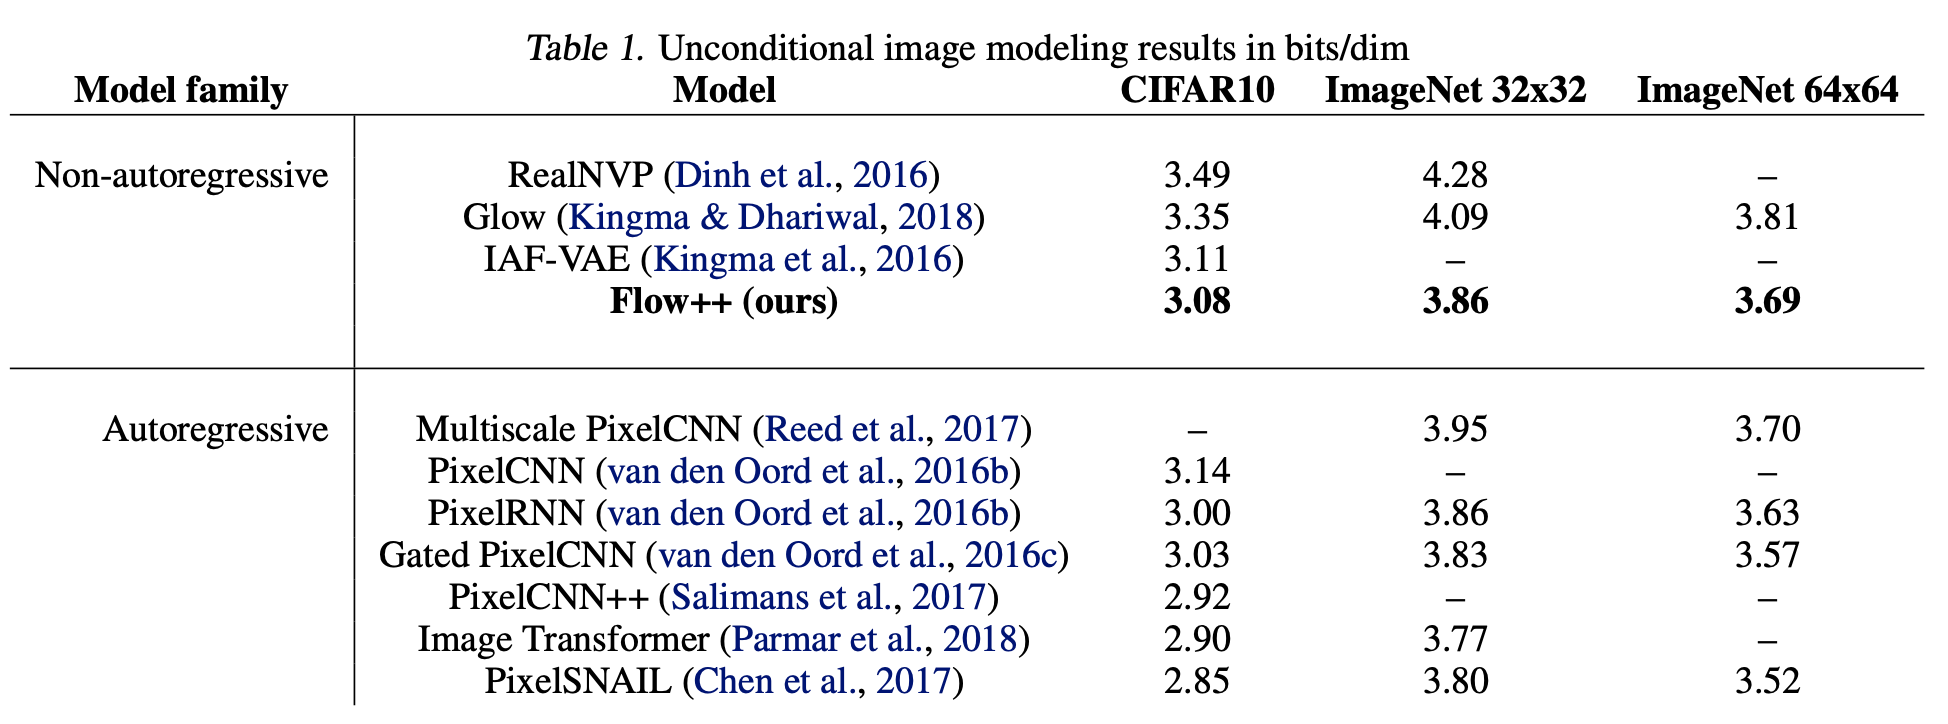
\includegraphics[width=0.7\linewidth]{figs/flow++1.png}
	\end{figure}
	\vspace{-0.1cm}
	\begin{figure}
		\centering
		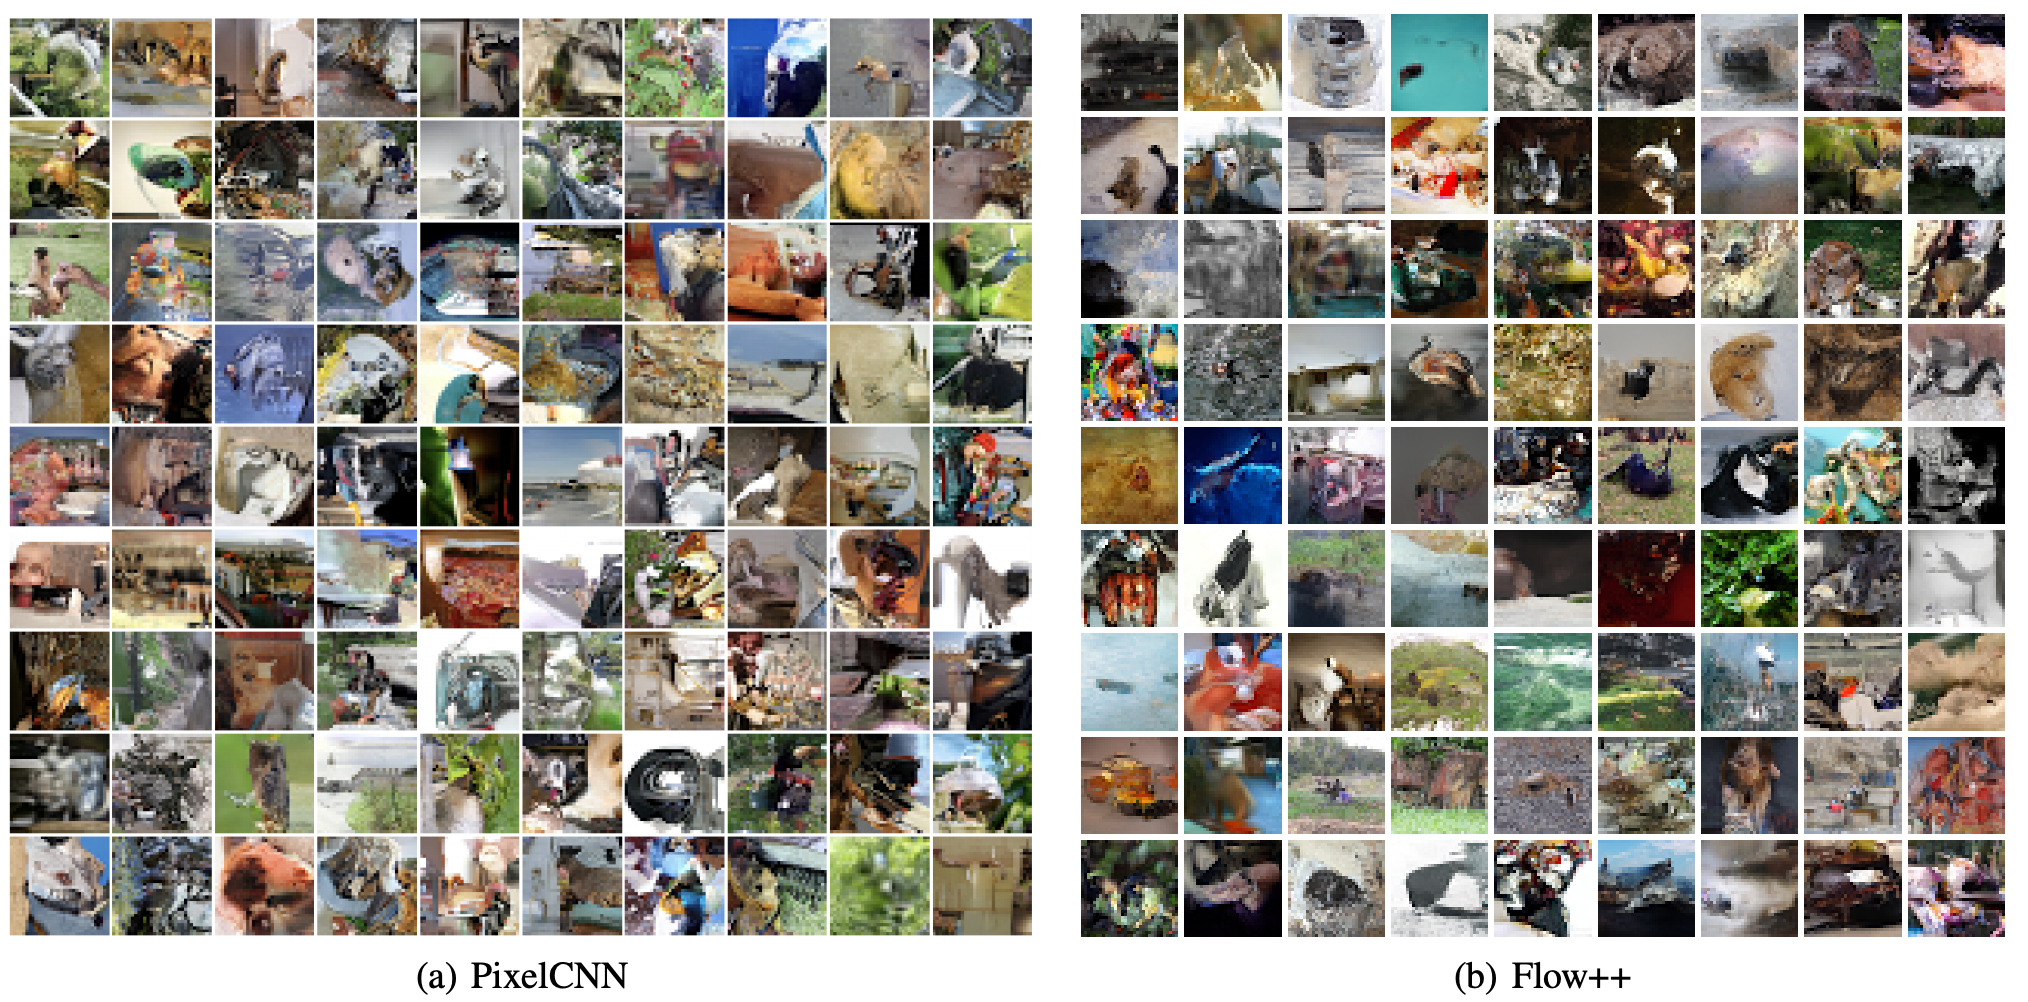
\includegraphics[width=0.8\linewidth]{figs/flow++2.png}
	\end{figure}
	\myfootnotewithlink{https://arxiv.org/abs/1902.00275}{Ho J. et al. Flow++: Improving Flow-Based Generative Models with Variational Dequantization and Architecture Design, 2019}
\end{frame}
%=======
\begin{frame}{VAE limitations}
	\begin{itemize}
		\item Poor variational posterior distribution (encoder)
		\[
		q(\bz | \bx, \bphi) = \mathcal{N}(\bz| \bmu_{\bphi}(\bx), \bsigma^2_{\bphi}(\bx)).
		\]
		\item Poor prior distribution
		\[
		p(\bz) = \mathcal{N}(0, \mathbf{I}).
		\]
		\item Poor probabilistic model (decoder)
		\[
		p(\bx | \bz, \btheta) = \mathcal{N}(\bx| \bmu_{\btheta}(\bz), \bsigma^2_{\btheta}(\bz)).
		\]
		\item Loose lower bound
		\[
		\log p(\bx | \btheta) - \mathcal{L}(q, \btheta) = (?).
		\]
	\end{itemize}
\end{frame}
%=======
\begin{frame}{Importance Sampling}
	\begin{block}{Generative model}
		\vspace{-0.5cm}
		\begin{align*}
			p(\bx | \btheta) &= \int p(\bx, \bz | \btheta) d\bz = \int \left[\frac{p(\bx, \bz | \btheta)}{q(\bz | \bx)} \right] q(\bz | \bx) d\bz \\
			&= \int f(\bx, \bz) q(\bz | \bx) d\bz = \mathbb{E}_{\bz \sim q(\bz | \bx)} f(\bx, \bz)
		\end{align*}
	\end{block}
	Here $f(\bx, \bz) = \frac{p(\bx, \bz | \btheta)}{q(\bz | \bx)}$.
	\begin{block}{ELBO}
		\vspace{-0.5cm}
		\begin{multline*}
			\log p(\bx | \btheta) = \log \mathbb{E}_{\bz \sim q(\bz | \bx)} f(\bx, \bz)
			\geq \mathbb{E}_{\bz \sim q(\bz | \bx)} \log f(\bx, \bz) = \\
			= \mathbb{E}_{\bz \sim q(\bz | \bx)} \log \frac{p(\bx, \bz | \btheta)}{q(\bz | \bx)} = \mathcal{L}(q, \btheta).
		\end{multline*}
	\end{block}
	Could we choose better $f(\bx, \bz)$? 
\end{frame}
%=======
\begin{frame}{IWAE}
	Let define
	\[
	f(\bx, \bz_1, \dots, \bz_K) = \frac{1}{K} \sum_{k=1}^K \frac{p(\bx, \bz_k | \btheta)}{q(\bz_k | \bx)}
	\]
	\[
		\mathbb{E}_{\bz_1, \dots, \bz_K \sim q(\bz | \bx)} f(\bx, \bz_1, \dots, \bz_K) = p(\bx | \btheta)
	\]
	\vspace{-0.3cm}
	\begin{block}{ELBO}
		\vspace{-0.5cm}
		\begin{multline*}
			\log p(\bx | \btheta) = \log \mathbb{E}_{\bz_1, \dots, \bz_K \sim q(\bz | \bx)} f(\bx, \bz, \dots, \bz_K) \geq \\
			\geq \mathbb{E}_{\bz_1, \dots, \bz_K \sim q(\bz | \bx)} \log f(\bx, \bz, \dots, \bz_K) = \\
			= \mathbb{E}_{\bz_1, \dots, \bz_K \sim q(\bz | \bx)} \log \left[\frac{1}{K} \sum_{k=1}^K\frac{p(\bx, \bz_k | \btheta)}{q(\bz_k | \bx)} \right] = \mathcal{L}_K(q, \btheta).
		\end{multline*}
	\end{block}
	\myfootnotewithlink{https://arxiv.org/abs/1509.00519}{Burda Y., Grosse R., Salakhutdinov R. Importance Weighted Autoencoders, 2015}
\end{frame}
%=======
\begin{frame}{IWAE}
	\begin{block}{VAE objective}
		\vspace{-0.2cm}
		\[
		\log p(\bx | \btheta) \geq \mathcal{L} (q, \btheta)  = \mathbb{E}_{q(\bz | \bx)} \log \frac{p(\bx, \bz | \btheta)}{q(\bz| \bx)} \rightarrow \max_{\bphi, \btheta}
		\]
		\[
		\mathcal{L} (q, \btheta)  = \mathbb{E}_{\bz_1, \dots, \bz_K \sim q(\bz | \bx)} \left( \frac{1}{K} \sum_{k=1}^K \log \frac{p(\bx, \bz_k | \btheta)}{q(\bz_k| \bx)} \right) \rightarrow \max_{q, \btheta}.
		\]
		\vspace{-0.2cm}
	\end{block}
	\begin{block}{IWAE objective}
		\vspace{-0.2cm}
		\[
		\mathcal{L}_K (q, \btheta)  = \mathbb{E}_{\bz_1, \dots, \bz_K \sim q(\bz | \bx)} \log \left( \frac{1}{K}\sum_{k=1}^K\frac{p(\bx, \bz_k | \btheta)}{q(\bz_k| \bx)} \right) \rightarrow \max_{q, \btheta}.
		\]
	\end{block}
	If $K=1$, these objectives coincide.

	\myfootnotewithlink{https://arxiv.org/abs/1509.00519}{Burda Y., Grosse R., Salakhutdinov R. Importance Weighted Autoencoders, 2015}
\end{frame}
%=======
\begin{frame}{IWAE}
	\begin{block}{Theorem}
		\begin{enumerate}
			\item $\log p(\bx | \btheta) \geq \mathcal{L}_K (q, \btheta) \geq \mathcal{L}_M (q, \btheta), \quad \text{for } K \geq M$;
			\item $\log p(\bx | \btheta) = \lim_{K \rightarrow \infty} \mathcal{L}_K (q, \btheta)$ if $\frac{p(\bx, \bz | \btheta)}{q(\bz | \bx)}$ is bounded.
		\end{enumerate}
		\vspace{-0.2cm}
	\end{block}
	\begin{block}{Proof of 1.}
		{ \footnotesize
			\vspace{-0.5cm}
			\begin{align*}
				\mathcal{L}_K (q, \btheta) &= \mathbb{E}_{\bz_1, \dots, \bz_K} \log \left( \frac{1}{K}\sum_{k=1}^K\frac{p(\bx, \bz_k | \btheta)}{q(\bz_k| \bx)} \right) = \\
				&= \mathbb{E}_{\bz_1, \dots, \bz_K} \log \mathbb{E}_{k_1, \dots, k_M} \left( \frac{1}{M}\sum_{m=1}^M\frac{p(\bx, \bz_{k_m} | \btheta)}{q(\bz_{k_m}| \bx)} \right) \geq \\
				&\geq \mathbb{E}_{\bz_1, \dots, \bz_K} \mathbb{E}_{k_1, \dots, k_m} \log \left( \frac{1}{M}\sum_{m=1}^M\frac{p(\bx, \bz_{k_m} | \btheta)}{q(\bz_{k_m}| \bx)} \right) = \\
				&= \mathbb{E}_{\bz_1, \dots, \bz_M} \log \left( \frac{1}{M}\sum_{m=1}^M\frac{p(\bx, \bz_m | \btheta)}{q(\bz_m| \bx)} \right) = \mathcal{L}_M (q, \btheta)
			\end{align*}
			\[
			\frac{a_1 + \dots + a_K}{K} = \mathbb{E}_{i_1, \dots, i_M} \frac{a_{i_1} + \dots + a_{i_M}}{M}, \quad i_1, \dots, i_M \sim U[1, K]
			\]
		}
	\end{block}
	
	\myfootnotewithlink{https://arxiv.org/abs/1509.00519}{Burda Y., Grosse R., Salakhutdinov R. Importance Weighted Autoencoders, 2015}
\end{frame}
%=======
\begin{frame}{IWAE}
	\begin{block}{Theorem}
		\begin{enumerate}
			\item $\log p(\bx | \btheta) \geq \mathcal{L}_K (q, \btheta) \geq \mathcal{L}_M (q, \btheta), \quad \text{for} K \geq M$;
			\item $\log p(\bx | \btheta) = \lim_{K \rightarrow \infty} \mathcal{L}_K (q, \btheta)$ if $\frac{p(\bx, \bz | \btheta)}{q(\bz | \bx)}$ is bounded.
		\end{enumerate}
		\vspace{-0.2cm}
	\end{block}
	\begin{block}{Proof of 2.}
		\vspace{0.2cm}
		Consider r.v. $\xi_K = \frac{1}{K}\sum_{k=1}^K \frac{p(\bx, \bz_k | \btheta)}{q(\bz_k | \bx)}$. \\
		\vspace{0.2cm}
		If summands are bounded, then (from the strong law of large numbers)
		\[
		\xi_K \xrightarrow[K \rightarrow \infty]{a.s.} \mathbb{E}_{q(\bz | \bx)} \frac{p(\bx, \bz | \btheta)}{q(\bz | \bx)} = p(\bx | \btheta).
		\]
		Hence $\mathcal{L}_K (q, \btheta) = \mathbb{E} \log \xi_K$ converges to $\log p(\bx | \btheta)$ as $K \rightarrow \infty$.
	\end{block}

	\myfootnotewithlink{https://arxiv.org/abs/1509.00519}{Burda Y., Grosse R., Salakhutdinov R. Importance Weighted Autoencoders, 2015}
\end{frame}
%=======
\begin{frame}{IWAE}
	\[
	\log p(\bx | \btheta) \geq \mathcal{L}_K(q, \btheta) \geq \mathcal{L}(q, \btheta)
	\]
	If $K > 1$ the bound could be tighter.
	\begin{align*}
		\mathcal{L} (q, \btheta) &= \mathbb{E}_{q(\bz | \bx)} \log \frac{p(\bx, \bz | \btheta)}{q(\bz| \bx)}; \\
		\mathcal{L}_K (q, \btheta) &= \mathbb{E}_{\bz_1, \dots, \bz_K \sim q(\bz | \bx)} \log \left( \frac{1}{K}\sum_{k=1}^K\frac{p(\bx, \bz_k | \btheta)}{q(\bz_k| \bx)} \right).
	\end{align*}
	\vspace{-0.2cm}
	\begin{itemize}
		\item $\mathcal{L}_1(q, \btheta) = \mathcal{L}(q, \btheta)$;
		\item $\mathcal{L}_{\infty}(q, \btheta) = \log p(\bx | \btheta)$.
	\end{itemize}
	\vspace{0.2cm}
	Which $q(\bz | \bx)$ gives $\mathcal{L}(q, \btheta) = \log p(\bx | \btheta)$? \\
	\vspace{0.2cm}
	Which $q(\bz | \bx)$ gives $\mathcal{L}(q, \btheta) = \mathcal{L}_K(q, \btheta)$?

	\myfootnotewithlink{https://arxiv.org/abs/1509.00519}{Burda Y., Grosse R., Salakhutdinov R. Importance Weighted Autoencoders, 2015}
\end{frame}
%=======
\begin{frame}{IWAE}
	\begin{block}{Theorem}
		The VAE objective is equal to IWAE objective 
		\[
		\mathcal{L}(q_{EW}, \btheta) = \mathcal{L}_K(q, \btheta)
		\]
		for the following variational distribution
		\[
		q_{EW}(\bz | \bx) = \mathbb{E}_{\bz_2, \dots, \bz_K \sim q(\bz | \bx)} q_{IW}(\bz | \bx, \bz_{2:K}),
		\]
		where \[
		q_{IW}(\bz | \bx, \bz_{2:K}) = \frac{\frac{p(\bx, \bz)}{q(\bz | \bx)}}{\frac{1}{K} \sum_{k=1}^K \frac{p(\bx, \bz_k)}{q(\bz_k | \bx)}} q(\bz | \bx) = \frac{p(\bx, \bz)}{\frac{1}{K}\left( \frac{p(\bx, \bz)}{q(\bz | \bx)} + \sum_{k=2}^K \frac{p(\bx, \bz_k)}{q(\bz_k | \bx)}\right)}.
		\]
	\end{block}
	
	\myfootnotewithlink{https://arxiv.org/abs/1704.02916}{Cremer C., Morris Q., Duvenaud D. Reinterpreting Importance-Weighted Autoencoders, 2017}
\end{frame}
%=======
\begin{frame}{IWAE}
	\begin{block}{IWAE posterior}
		\vspace{-0.3cm}
		\begin{figure}
			\centering
			\includegraphics[width=\linewidth]{figs/IWAE_1.png}
		\end{figure}
	\end{block}
	\vspace{-0.5cm}
	\begin{block}{IWAE samples}
		\vspace{-0.3cm}
		\begin{figure}
			\centering
			\includegraphics[width=\linewidth]{figs/IWAE_2.png}
		\end{figure}
	\end{block}

	\myfootnotewithlink{https://arxiv.org/abs/1704.02916}{Cremer C., Morris Q., Duvenaud D. Reinterpreting Importance-Weighted Autoencoders, 2017}
\end{frame}
%=======
\begin{frame}{IWAE}
	\begin{block}{Objective}
		\vspace{-0.5cm}
		\[
		\mathcal{L}_K (q, \btheta)  = \mathbb{E}_{\bz_1, \dots, \bz_K \sim q(\bz | \bx, \bphi)} \log \left( \frac{1}{K}\sum_{k=1}^K\frac{p(\bx, \bz_k | \btheta)}{q(\bz_k| \bx, \bphi)} \right) \rightarrow \max_{\bphi, \btheta}.
		\]
		\vspace{-0.3cm}
	\end{block}
	\begin{block}{Gradient}
		\vspace{-0.3cm}
		\[
		\Delta_K = \nabla_{\btheta, \bphi} \log \left( \frac{1}{K}\sum_{k=1}^K\frac{p(\bx, \bz_k | \btheta)}{q(\bz_k| \bx, \bphi)} \right), \quad \bz_k \sim q(\bz | \bx, \bphi).
		\]
		\vspace{-0.3cm}
	\end{block}
	\begin{block}{Theorem}
		\vspace{-0.4cm}
		\[
			\text{SNR}_K = \frac{\bbE [\Delta_K]}{\sigma(\Delta_K)}; \quad
			\text{SNR}_K(\btheta) = O(\sqrt{K}); \quad 
			\text{SNR}_K(\bphi) = O\left(\sqrt{\frac{1}{K}}\right).
		\]
		Hence, increasing $K$ vanishes gradient signal of inference network $q(\bz | \bx, \bphi)$.
	\end{block}

	\myfootnotewithlink{https://arxiv.org/abs/1802.04537}{Rainforth T. et al. Tighter variational bounds are not necessarily better, 2018}
\end{frame}
%=======
\begin{frame}{IWAE}
	\begin{block}{Theorem}
		\vspace{-0.5cm}
		\[
			\text{SNR}_K = \frac{\bbE [\Delta_K]}{\sigma(\Delta_K)}; \quad
			\text{SNR}_K(\btheta) = O(\sqrt{K}); \quad 
			\text{SNR}_K(\bphi) = O\left(\sqrt{\frac{1}{K}}\right).
		\]
		\vspace{-0.8cm}
	\end{block}
		\begin{minipage}[t]{0.5\columnwidth}
			\begin{figure}[h]
				\centering
				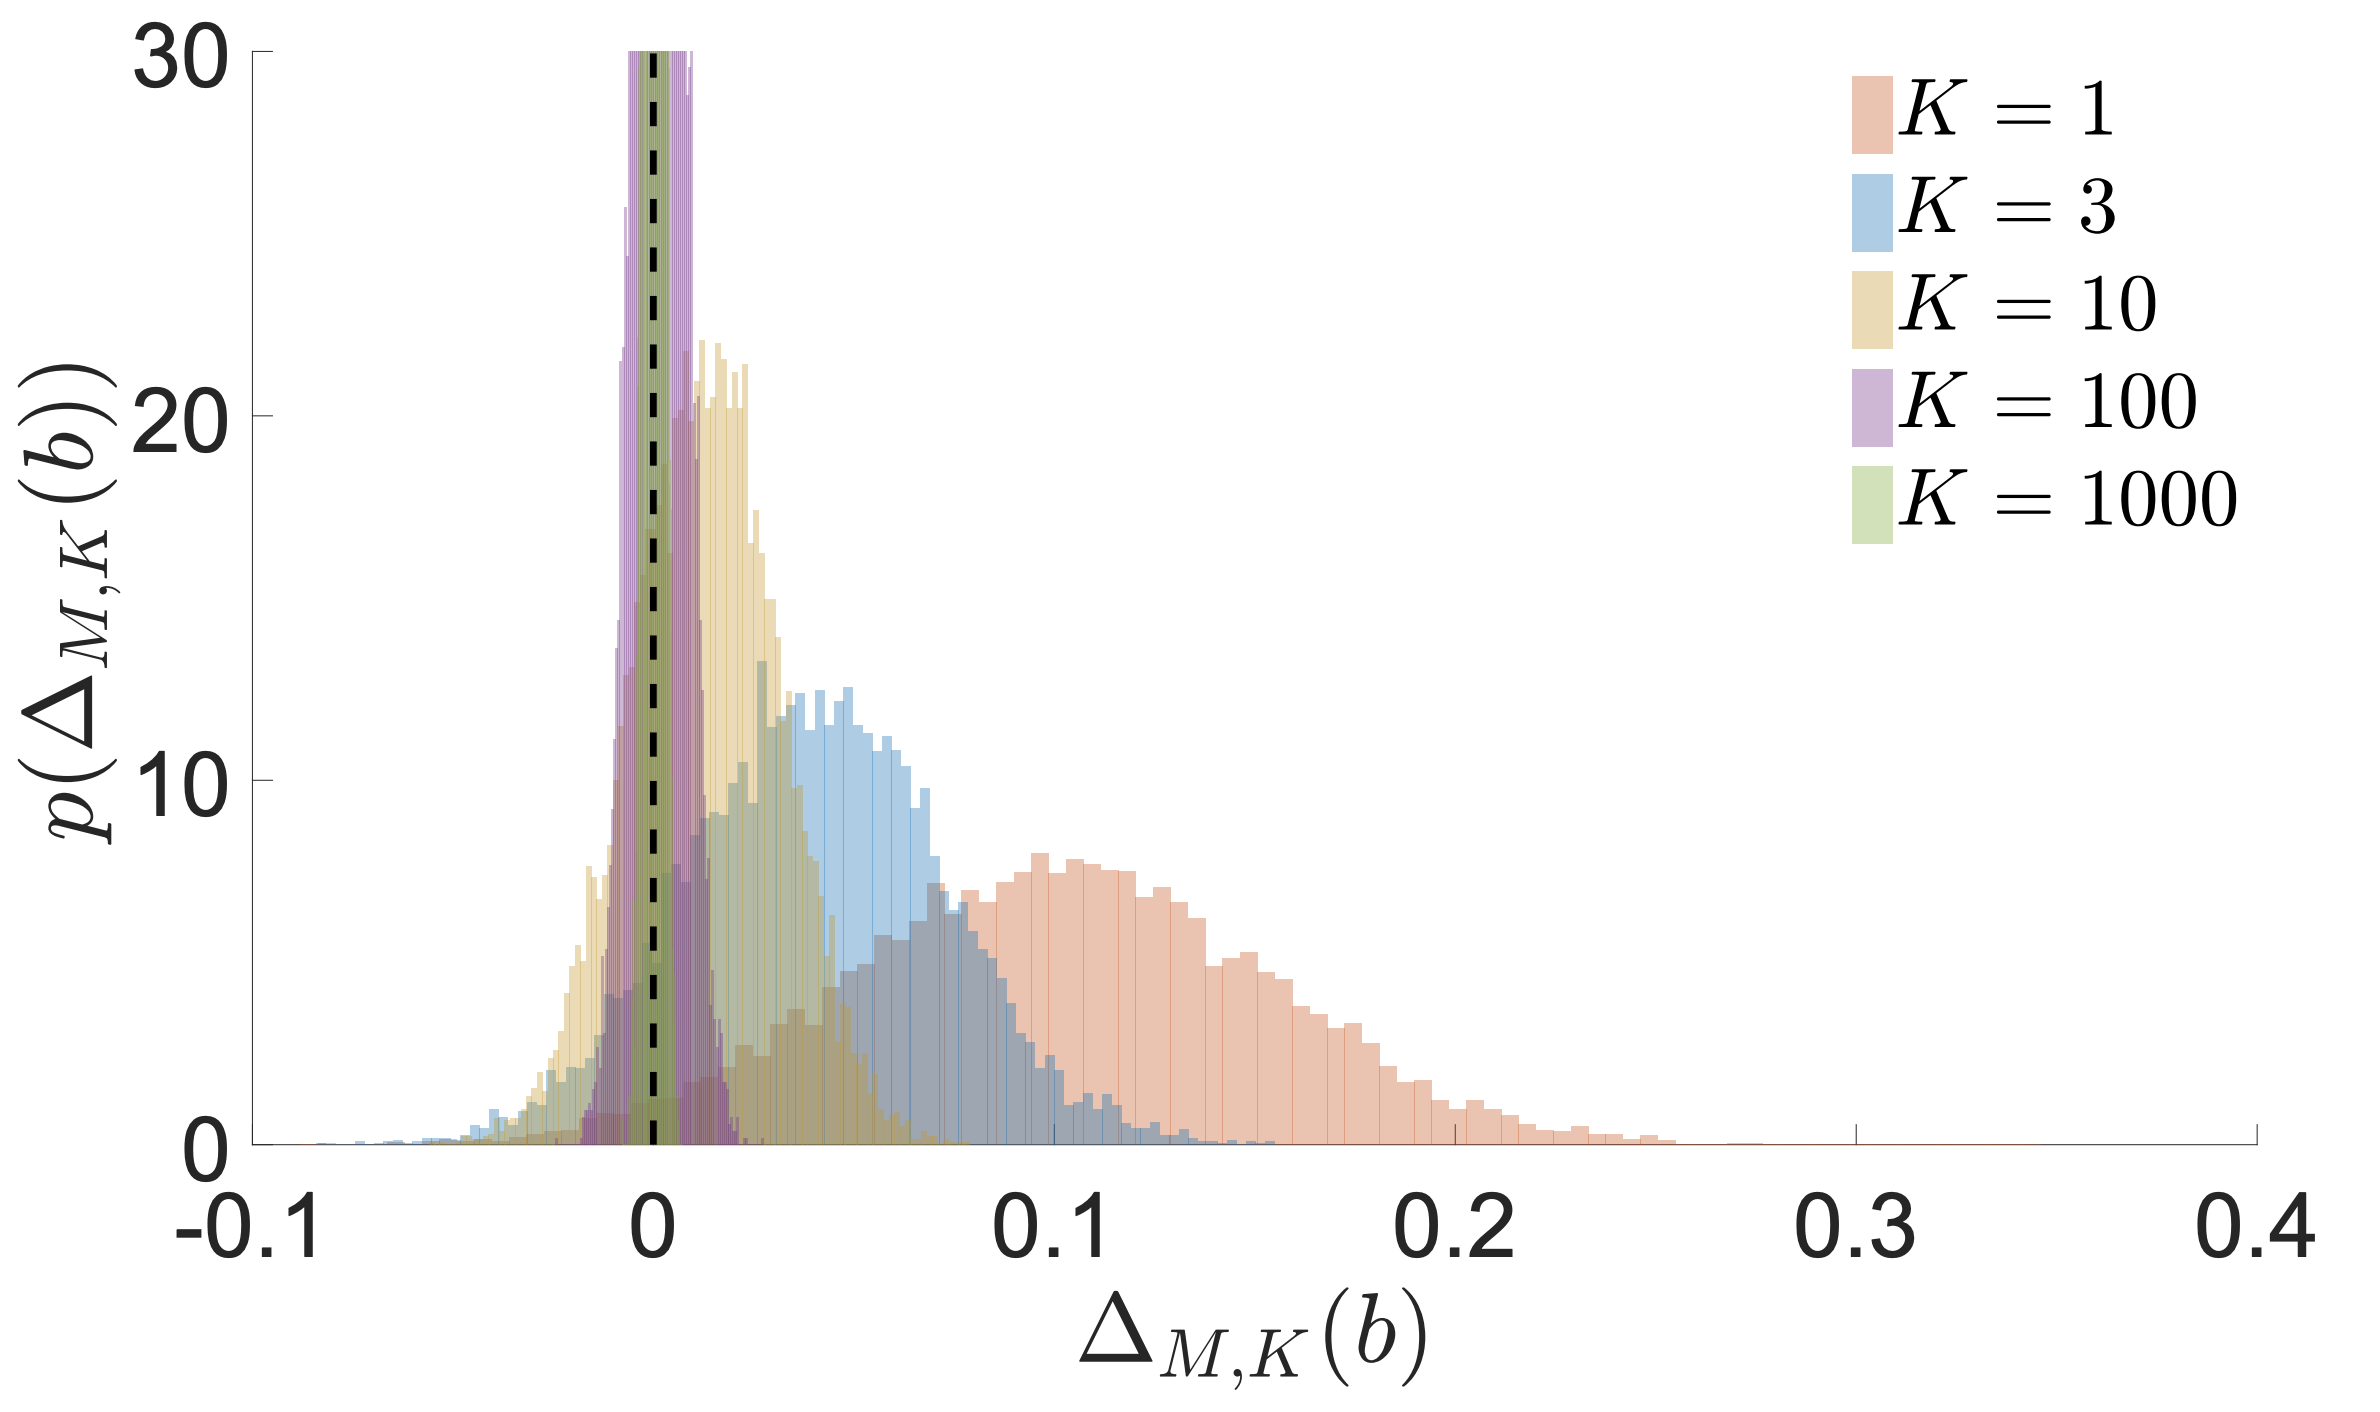
\includegraphics[width=1.\linewidth]{figs/IWAE_SNR_1.png}
			\end{figure}
		\end{minipage}%
		\begin{minipage}[t]{0.5\columnwidth}
			\begin{figure}[h]
				\centering
				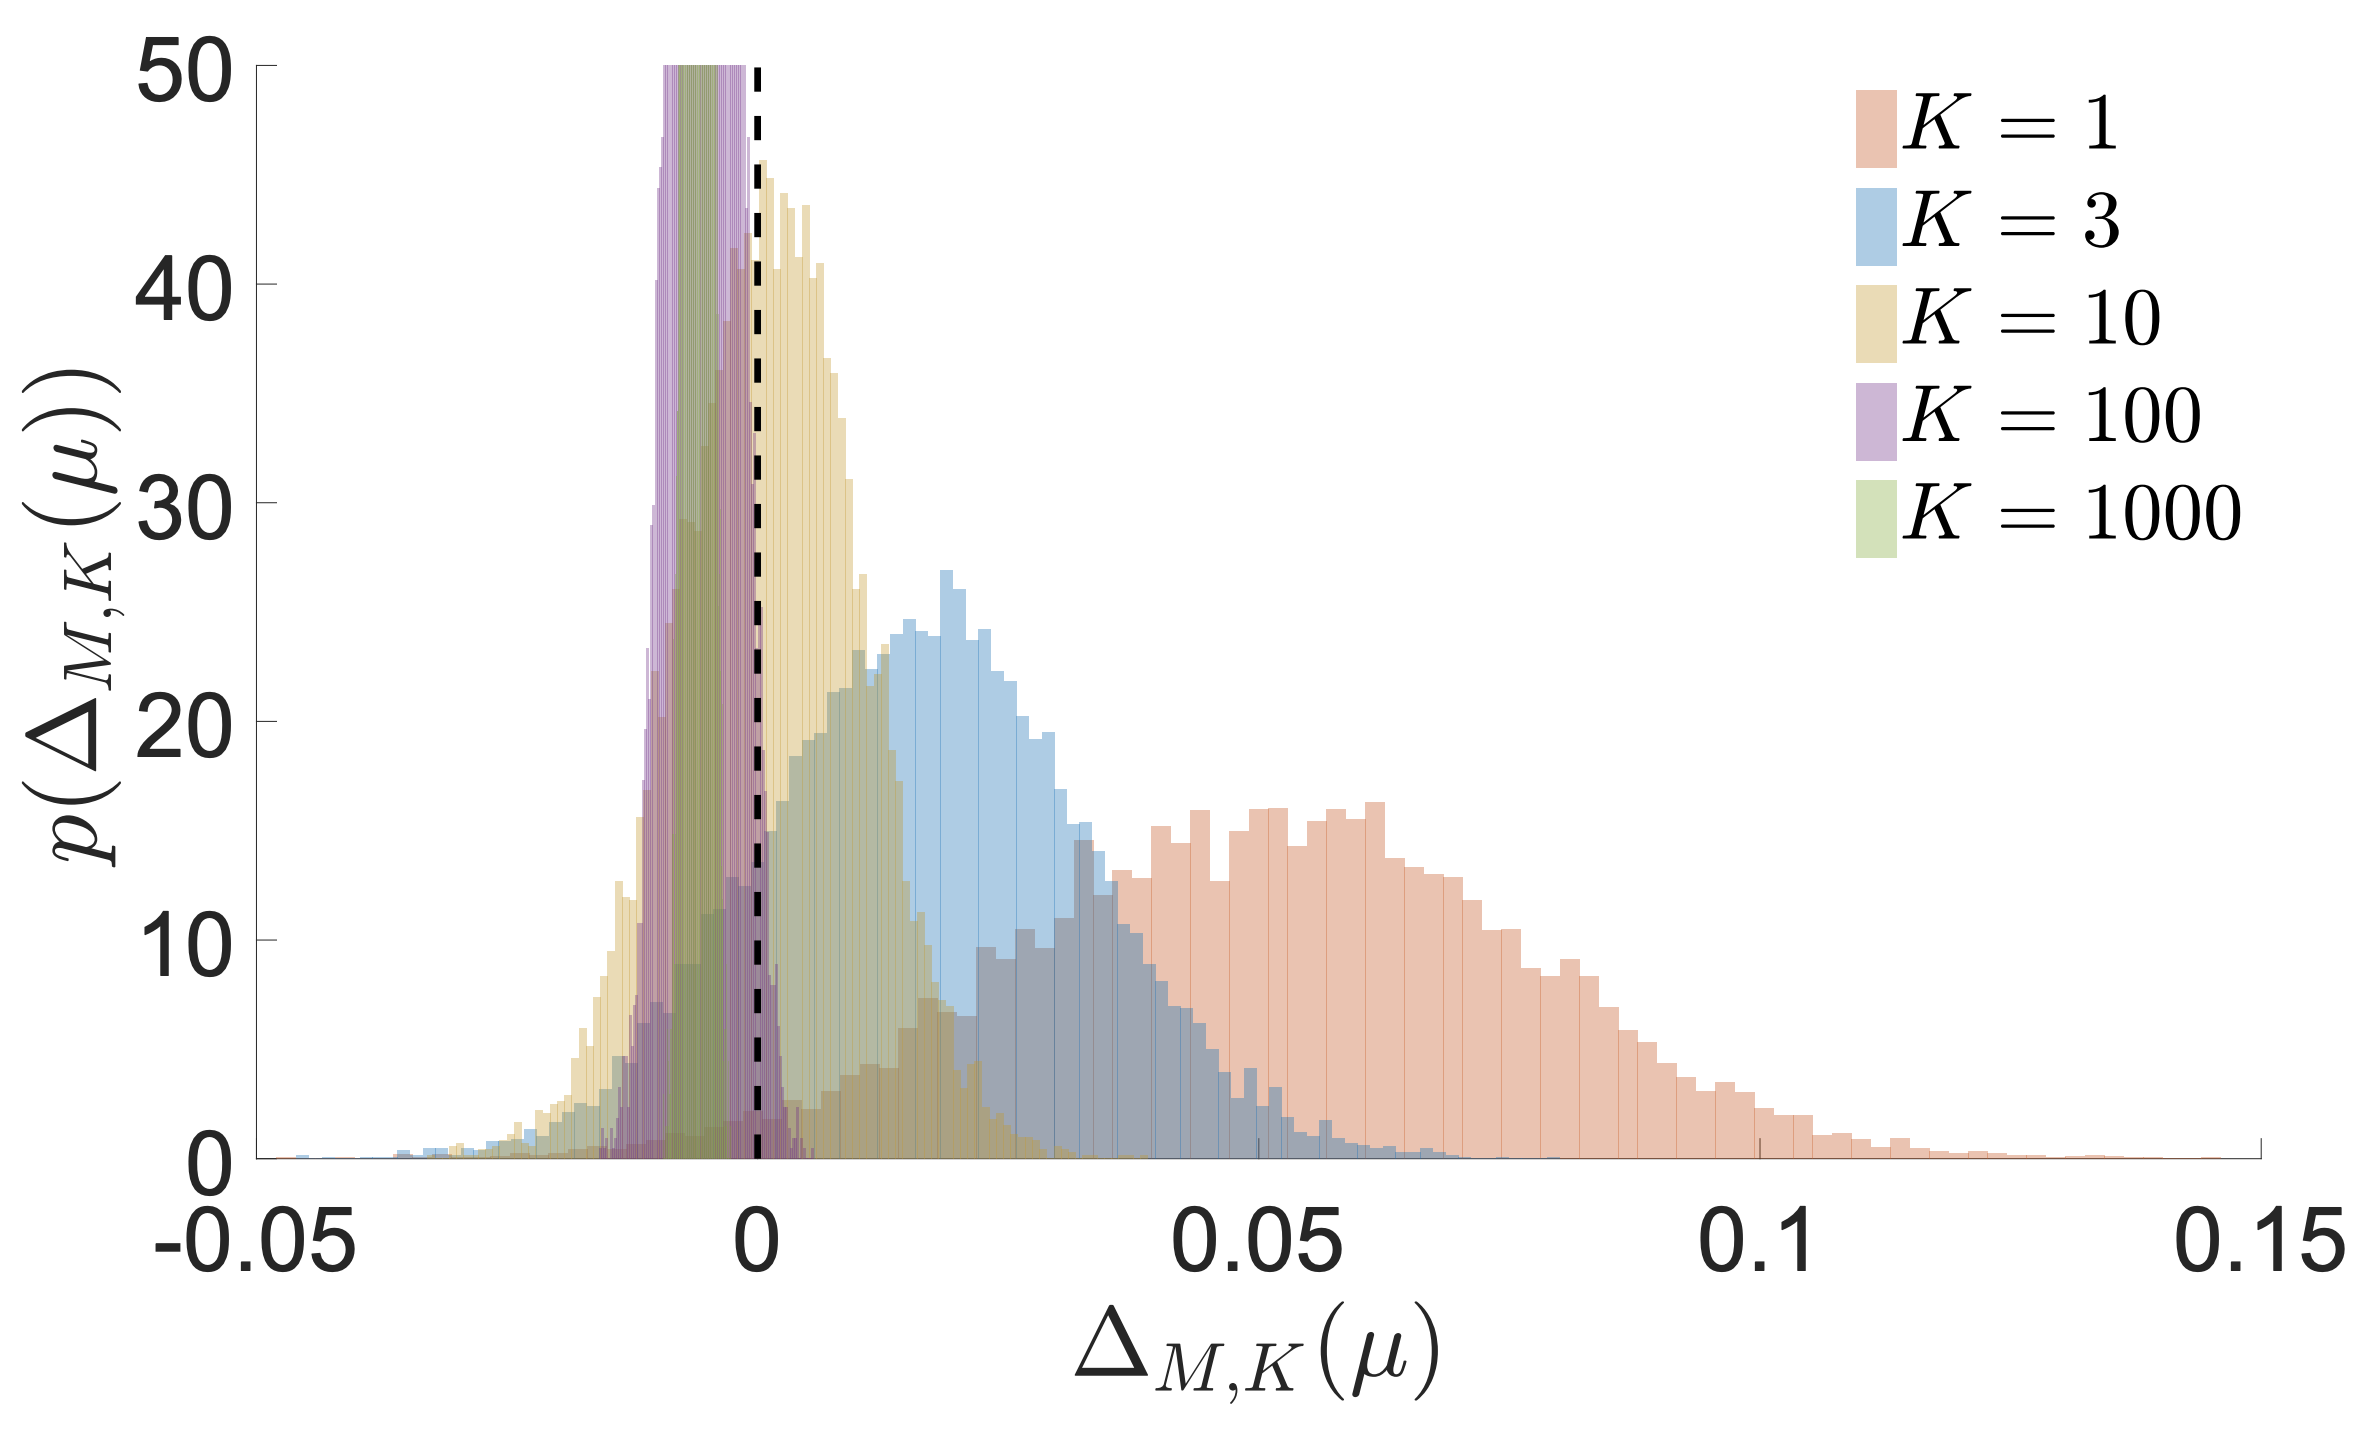
\includegraphics[width=1.\linewidth]{figs/IWAE_SNR_2.png}
			\end{figure}
		\end{minipage}
	\begin{itemize}
		\item IWAE makes the variational bound tighter and extends the class of variational distributions.
		\item Gradient signal becomes really small, training is complicated.
		\item IWAE is very popular technique as a quality measure for VAE models.
	\end{itemize}
	\myfootnotewithlink{https://arxiv.org/abs/1802.04537}{Rainforth T. et al. Tighter variational bounds are not necessarily better, 2018}
\end{frame}
%=======
\begin{frame}{VAE limitations}
	\begin{itemize}
		\item Poor variational posterior distribution (encoder)
		\[
			q(\bz | \bx, \bphi) = \mathcal{N}(\bz| \bmu_{\bphi}(\bx), \bsigma^2_{\bphi}(\bx)).
		\]
		\item Poor prior distribution
		\[
			p(\bz) = \mathcal{N}(0, \mathbf{I}).
		\]
		\item Poor probabilistic model (decoder)
		\[
			p(\bx | \bz, \btheta) = \mathcal{N}(\bx| \bmu_{\btheta}(\bz), \bsigma^2_{\btheta}(\bz)).
		\]
		\item Loose lower bound
		\[
			\log p(\bx | \btheta) - \mathcal{L}(q, \btheta) = (?).
		\]
	\end{itemize}
\end{frame}
%=======
\begin{frame}{ELBO interpretations}
	\[
		\log p(\bx | \btheta) = \cL (\bphi, \btheta) + KL(q(\bz | \bx, \bphi) || p(\bz | \bx, \btheta)) \geq  \cL (\bphi, \btheta).
	\]
	\[
		\cL (\bphi, \btheta) = \int q(\bz | \bx, \bphi) \log \frac{p(\bx, \bz | \btheta)}{q(\bz | \bx, \bphi)} d \bz.
	\]
	\begin{itemize}
	    \item Evidence minus posterior KL
	    \vspace{-0.1cm}
	    \[
	        \mathcal{L}(q, \btheta) = \log p(\bx | \btheta) - KL(q(\bz | \bx, \bphi) || p(\bz | \bx, \btheta)).
	    \]
	    \item Average negative energy plus entropy
	    \vspace{-0.1cm}
	    \begin{align*}
	        \mathcal{L}(q, \btheta) &= \mathbb{E}_{q(\bz | \bx, \bphi)} \left[\log p(\bx, \bz | \btheta) - \log q(\bz | \bx, \bphi)  \right] \\
	        &= \mathbb{E}_{q(\bz | \bx, \bphi)} \log p(\bx, \bz | \btheta) + \mathbb{H} \left[q(\bz | \bx, \bphi) \right].
	    \end{align*}
	    \item Average reconstruction minus KL to prior
	    \vspace{-0.1cm}
	    \begin{align*}
	        \mathcal{L}(q, \btheta) &= \mathbb{E}_{q(\bz | \bx, \bphi)} \left[ \log p(\bx | \bz, \btheta) + \log p(\bz) - \log q(\bz | \bx, \bphi) \right] \\
	        &= \mathbb{E}_{q(\bz | \bx, \bphi)} \log p(\bx | \bz, \btheta) - KL(q(\bz | \bx, \bphi) || p(\bz)).
	    \end{align*}
	\end{itemize}
\end{frame}
%=======
\begin{frame}{ELBO surgery, 2016}
	\vspace{-0.3cm}
	\[
	    \sum_{i=1}^n \mathcal{L}_i(q, \btheta) = \frac{1}{n} \sum_{i=1}^n \left[ \mathbb{E}_{q(\bz_i | \bx_i)} \log p(\bx_i | \bz_i, \btheta) - KL(q(\bz_i | \bx_i) || p(\bz_i)) \right].
	\]
	\vspace{-0.3cm}
	\begin{block}{Theorem}
	\[
	    \frac{1}{n} \sum_{i=1}^n KL(q(\bz_i | \bx_i) || p(\bz_i)) = KL(q(\bz) || p(\bz)) + \bbI_{q(i, \bz)} [i, \bz],
	\]
	where $i$ is treated as random variable:
	\footnotesize{
	\[
	    q(i, \bz) = q(i) q(\bz | i); \quad p(i, \bz) = p(i) p(\bz); \quad 
	    q(i) = p(i) = \frac{1}{n}; \quad q(\bz | i) = q(\bz | \bx_i).
	\]
	\[
	    q(\bz) = \sum_{i=1}^n q(i, \bz) = \frac{1}{n} \sum_{i=1}^n q(\bz | \bx_i); \quad  \mathbb{I}_{q(i, \bz)} [i, \bz] = \mathbb{E}_{q(i, \bz)} \log \frac{q(i, \bz)}{q(i)q(\bz)}.
	\]
	}
	\end{block}
	\myfootnotewithlink{http://approximateinference.org/accepted/HoffmanJohnson2016.pdf}{Hoffman M. D., Johnson M. J. ELBO surgery: yet another way to carve up the variational evidence lower bound, 2016}
\end{frame}
%=======
\begin{frame}{ELBO surgery, 2016}
	\begin{block}{Theorem}
	\[
	    \frac{1}{n} \sum_{i=1}^n KL(q(\bz_i | \bx_i) || p(\bz_i)) = KL(q(\bz) || p(\bz)) + \mathbb{I}_{q(i, \bz)} [i, \bz].
	\]
	\end{block}
	\begin{block}{Proof}
	\vspace{-0.3cm}
	{\footnotesize
	\begin{multline*}
	    \frac{1}{n} \sum_{i=1}^n KL(q(\bz_i | \bx_i) || p(\bz_i)) = \sum_{i=1}^n \int q(i) q(\bz | i) \log \frac{q(\bz | i)}{p(\bz)} d \bz = \\
	    = \sum_{i=1}^n \int q(i, \bz) \log \frac{q(i, \bz)}{p(\bz)p(i)} d \bz =
	    \int \sum_{i=1}^n q(i, \bz) \log \frac{ q (\bz) q(i | \bz) }{p(\bz) p(i) } d \bz = \\
	    = \int q(\bz) \log \frac{q(\bz)}{p(\bz)} d\bz + \int \sum_{i=1}^n q(i | \bz) q(\bz) \log \frac{q(i | \bz)}{p(i)} d \bz = \\
	    = KL (q(\bz) || p(\bz)) - \mathbb{E}_{q(\bz)} \mathbb{H} \left[q(i | \bz)  \right] + \log n.
	\end{multline*}
	}
	\end{block}

	\myfootnotewithlink{http://approximateinference.org/accepted/HoffmanJohnson2016.pdf}{Hoffman M. D., Johnson M. J. ELBO surgery: yet another way to carve up the variational evidence lower bound, 2016}
\end{frame}
%=======
\begin{frame}{ELBO surgery, 2016}
	\begin{block}{Theorem}
	\[
	    \frac{1}{n} \sum_{i=1}^n KL(q(\bz_i | \bx_i) || p(\bz_i)) = KL(q(\bz) || p(\bz)) + \mathbb{I}_{q(i, \bz)} [i, \bz].
	\]
	\end{block}
	\begin{block}{Proof (continued)}
	{\footnotesize
	\[
	    \frac{1}{n} \sum_{i=1}^n KL(q(\bz_i | \bx_i) || p(\bz_i)) = KL (q(\bz) || p(\bz)) - \mathbb{E}_{q(\bz)} \mathbb{H} \left[q(i | \bz) \right] + \log n
	\]
	\begin{multline*}
	    \mathbb{I}_{q(i, \bz)} [i, \bz] = \mathbb{E}_{q(i, \bz)} \log \frac{q(i, \bz)}{q(i)q(\bz)} = \mathbb{E}_{q(\bz)} \mathbb{E}_{q(i | \bz)} \log \frac{q(i | \bz) q(\bz)}{q(i)q(\bz)} = \\
	    = \mathbb{E}_{q(\bz)} \mathbb{E}_{q(i | \bz)} \log \frac{q(i | \bz)}{q(i)} = - \mathbb{E}_{q(\bz)} \mathbb{H} \left[ q(i | \bz) \right] + \log n.
	\end{multline*}
	}
	\end{block}

	\myfootnotewithlink{http://approximateinference.org/accepted/HoffmanJohnson2016.pdf}{Hoffman M. D., Johnson M. J. ELBO surgery: yet another way to carve up the variational evidence lower bound, 2016}
\end{frame}
%=======
\begin{frame}{ELBO surgery, 2016}
	\begin{block}{Theorem}
	\[
	    \frac{1}{n} \sum_{i=1}^n KL(q(\bz_i | \bx_i) || p(\bz_i)) = KL(q(\bz) || p(\bz)) + \mathbb{I}_{q(i, \bz)} [i, \bz].
	\]
	\end{block}
	\begin{block}{ELBO revisiting}
	{\footnotesize
	\begin{multline*}
	    \sum_{i=1}^n \cL_i(q, \btheta) = \frac{1}{n} \sum_{i=1}^n \left[ \mathbb{E}_{q(\bz_i | \bx_i)} \log p(\bx_i | \bz_i, \btheta) - KL(q(\bz_i | \bx_i) || p(\bz_i)) \right] = \\
	    = \frac{1}{n} \sum_{i=1}^n \mathbb{E}_{q(\bz_i | \bx_i)} \log p(\bx_i | \bz_i, \btheta) - \mathbb{I}_{q(i, \bz)} [i, \bz] - KL(q(\bz) || p(\bz)) = \\
	    = \underbrace{\frac{1}{n} \sum_{i=1}^n \mathbb{E}_{q(\bz_i | \bx_i)} \log p(\bx_i | \bz_i, \btheta)}_{\text{Reconstruction loss}} - \underbrace{\left(\log n - \mathbb{E}_{q(\bz)} \mathbb{H} \left[ q(i | \bz) \right] \right)\vphantom{\sum_{i=1}} }_{0 \leq \text{Mutual info} \leq \log n } - \underbrace{KL(q(\bz) || p(\bz))\vphantom{\sum_{i=1}}}_{\text{Marginal KL}}
	\end{multline*}
	}
	\end{block}

	\myfootnotewithlink{http://approximateinference.org/accepted/HoffmanJohnson2016.pdf}{Hoffman M. D., Johnson M. J. ELBO surgery: yet another way to carve up the variational evidence lower bound, 2016}
\end{frame}
%=======
\begin{frame}{ELBO surgery, 2016}
	\begin{block}{ELBO revisiting}
	\vspace{-0.7cm}
	{\footnotesize
	\begin{multline*}
	    \sum_{i=1}^n \mathcal{L}(q, \btheta) = \underbrace{\frac{1}{n} \sum_{i=1}^n \mathbb{E}_{q(\bz_i | \bx_i)} \log p(\bx_i | \bz_i, \btheta)}_{\text{Reconstruction loss}} - \\
	    - \underbrace{\left(\log n - \mathbb{E}_{q(\bz)} \mathbb{H} \left[ q(i | \bz) \right] \right)\vphantom{\sum_{i=1}}}_{0 \leq \text{Mutual info} \leq \log n } - \underbrace{KL(q(\bz) || p(\bz))\vphantom{\sum_{i=1}}}_{\text{Marginal KL}}
	\end{multline*}}
	\end{block}
	\vspace{-0.8cm}
	\[
	    KL(q(\bz) || p(\bz)) = 0 \quad \Leftrightarrow \quad p (\bz) = q(\bz) = \frac{1}{n} \sum_{i=1}^n q(\bz | \bx_i).
	\]
	\vspace{-0.3cm}
	\begin{figure}
	    \centering
	    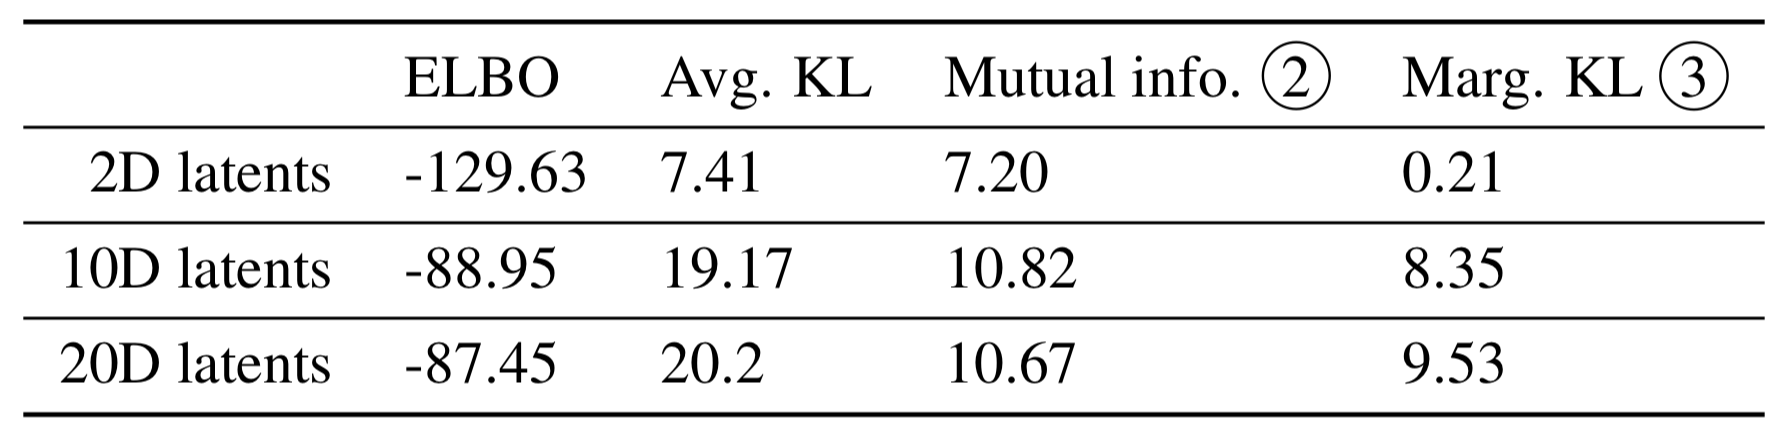
\includegraphics[width=0.7\linewidth]{figs/ELBO_surgery.png}
	\end{figure}
	\vspace{-0.3cm}
	\[
	\log n \approx 11.0021
	\]
	\myfootnotewithlink{http://approximateinference.org/accepted/HoffmanJohnson2016.pdf}{Hoffman M. D., Johnson M. J. ELBO surgery: yet another way to carve up the variational evidence lower bound, 2016}
\end{frame}
%=======
\begin{frame}{VAE prior}
	\vspace{-0.5cm}
	\begin{block}{ELBO revisiting}
	\vspace{-0.5cm}
	{\footnotesize
	\begin{multline*}
	    \sum_{i=1}^n \mathcal{L}(q, \btheta) = \underbrace{\frac{1}{n} \sum_{i=1}^n \mathbb{E}_{q(\bz_i | \bx_i)} \log p(\bx_i | \bz_i, \btheta)}_{\text{Reconstruction loss}} - \\
	    - \underbrace{\left(\log n - \mathbb{E}_{q(\bz)} \mathbb{H} \left[ q(i | \bz) \right] \right)\vphantom{\sum_{i=1}}}_{0 \leq \text{Mutual info} \leq \log n } - \underbrace{KL(q(\bz) || p(\bz))\vphantom{\sum_{i=1}}}_{\text{Marginal KL}}
	\end{multline*}}
	\end{block}
	\vspace{-0.4cm}
	
	How to choose the optimal $p(\bz)$?
	\begin{itemize}
	    \item SG: $p(\bz) = \mathcal{N}(0, I)$ $\Rightarrow$ over-regularization;
	    \vspace{0.1cm}
	    \item MoG: $p(\bz | \blambda) = \frac{1}{K} \sum_{k=1}^K \mathcal{N}(\bmu_k, \bsigma_k^2)$ $\Rightarrow$ (*), (**);
	    \vspace{0.1cm}
	    \item $p(\bz) = q(\bz) = \frac{1}{n}\sum_{i=1}^n q(\bz | \bx_i)$ $\Rightarrow$ overfitting and highly expensive.
	\end{itemize}

	\myfootnote{\href{https://arxiv.org/abs/1611.02648}{(*) Dilokthanakul N. et al. Deep Unsupervised Clustering with Gaussian Mixture Variational Autoencoders, 2016} \\
	\href{https://pdfs.semanticscholar.org/f6fe/5e8e25994c188ba6a124462e2cc55f2c5a67.pdf}{(**) Nalisnick E., Hertel L., Smyth P. Approximate Inference for Deep Latent Gaussian Mixtures, 2016}}

\end{frame}
%=======
\begin{frame}{VampPrior}
	\begin{block}{Variational Mixture of posteriors}
		\[
		p(\bz | \blambda) = \frac{1}{K} \sum_{k=1}^K q(\bz | \bu_k),
		\]
		where $\blambda = \{\bu_1, \dots, \bu_K\}$ are trainable preudo-inputs.
	\end{block}
	\begin{itemize}
		\item Multimodal $\Rightarrow$ prevents over-regularization;.
		\item $K \ll n$ $\Rightarrow$ prevents from potential overfitting + less expensive to train.
		\item Pseudo-inputs are prior hyperparameters $\Rightarrow$ connection to the Empirical Bayes.
	\end{itemize}
	\myfootnotewithlink{https://arxiv.org/abs/1705.07120}{Tomczak J. M., Welling M. VAE with a VampPrior, 2017}
\end{frame}
%=======
\begin{frame}{VampPrior}
	\begin{itemize}
	\item Do we equally need the multimodal prior?
	\item Is it beneficial to couple the prior with the variational posterior or MoG is enough?
	\end{itemize}
	\begin{block}{MNIST results}
		\begin{minipage}[t]{0.5\columnwidth}
			\begin{figure}[h]
				\centering
				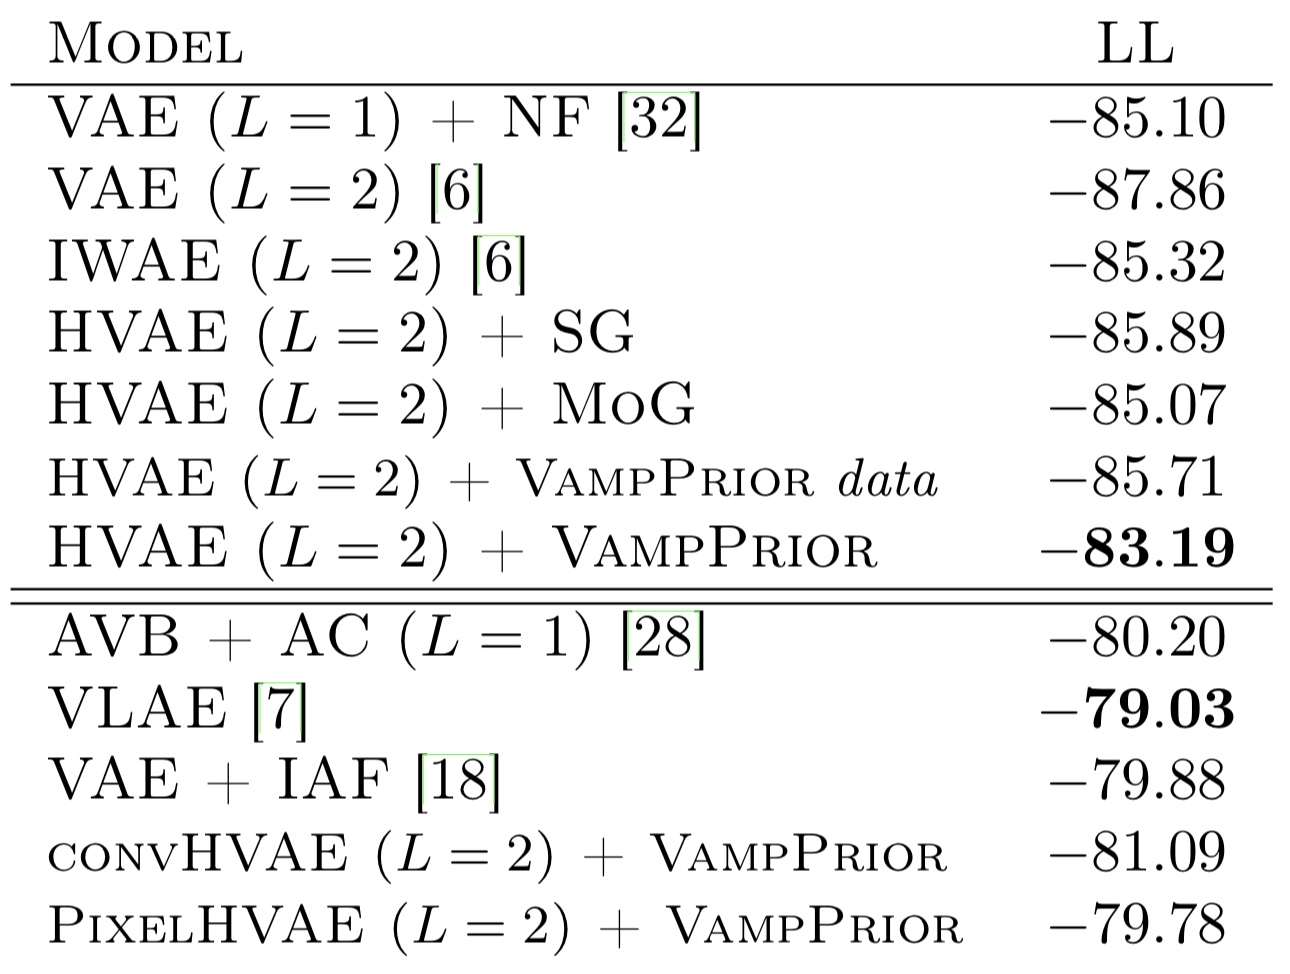
\includegraphics[width=0.9\linewidth]{figs/VampPrior_1.png}
			\end{figure}
		\end{minipage}%
		\begin{minipage}[t]{0.5\columnwidth}
			\begin{figure}[h]
				\centering
				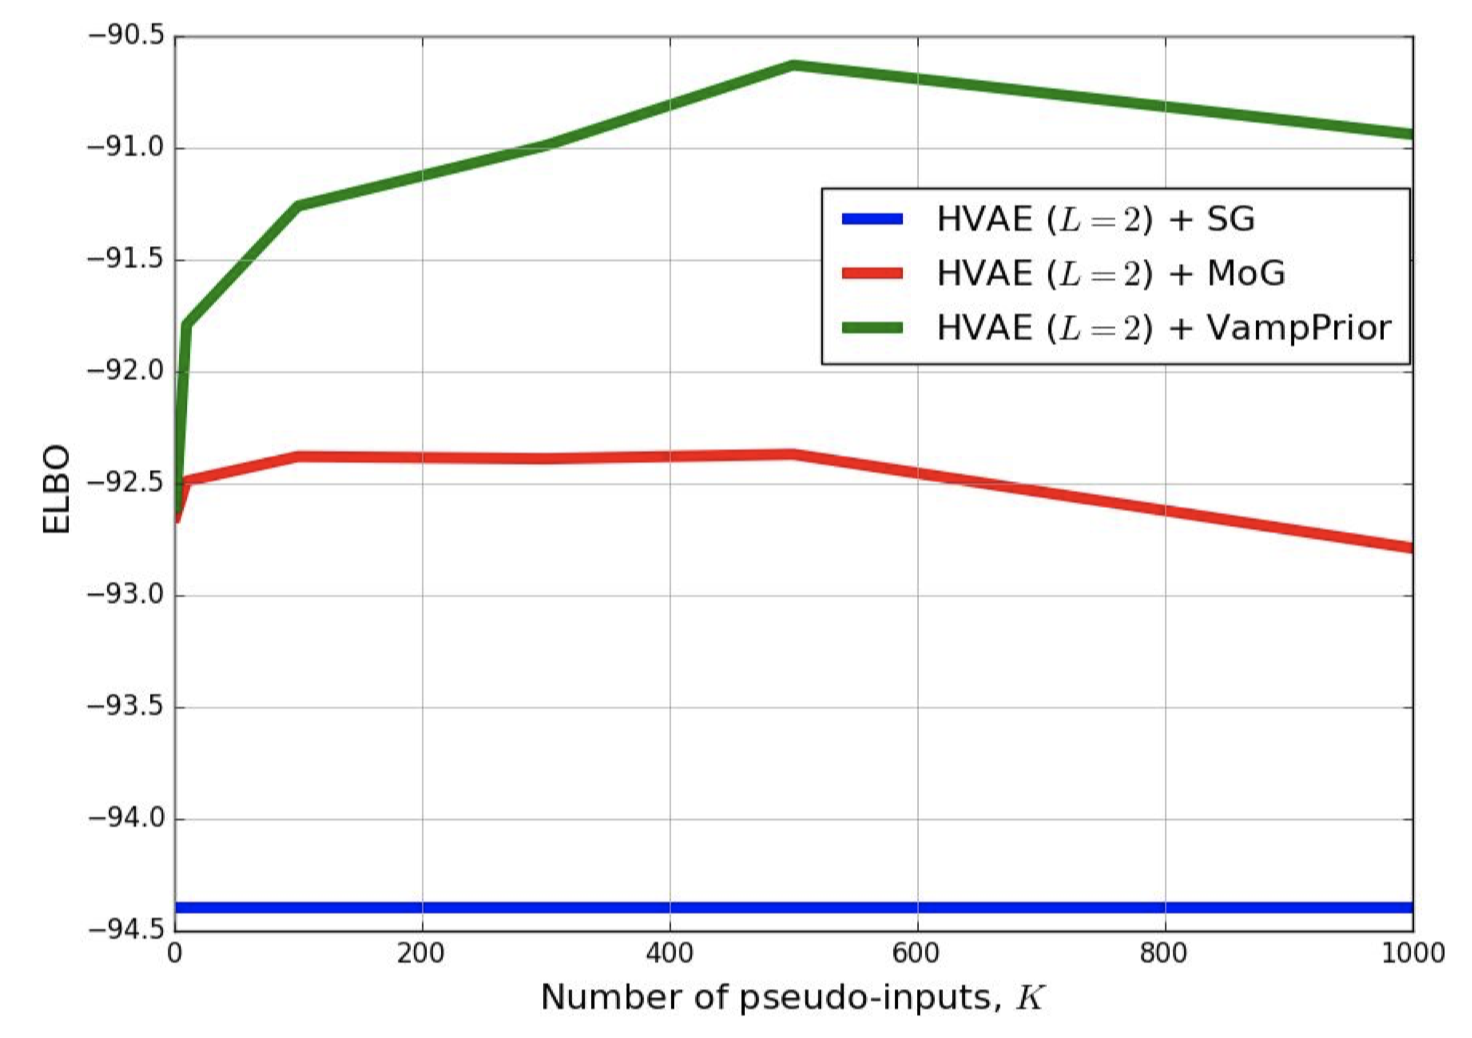
\includegraphics[width=1.\linewidth]{figs/VampPrior_2.png}
			\end{figure}
		\end{minipage}
	\end{block}
	\myfootnotewithlink{https://arxiv.org/abs/1705.07120}{Tomczak J. M., Welling M. VAE with a VampPrior, 2017}
\end{frame}
%=======
\begin{frame}{VampPrior}
	\vspace{0.1cm}
	\textbf{Top row:} generated images by PixelHVAE + VampPrior for chosen pseudo-input in the left top corner. \\
	\vspace{0.1cm}
	\textbf{Bottom row:} pseudo-inputs for different datasets.
	\begin{figure}[h]
		\centering
		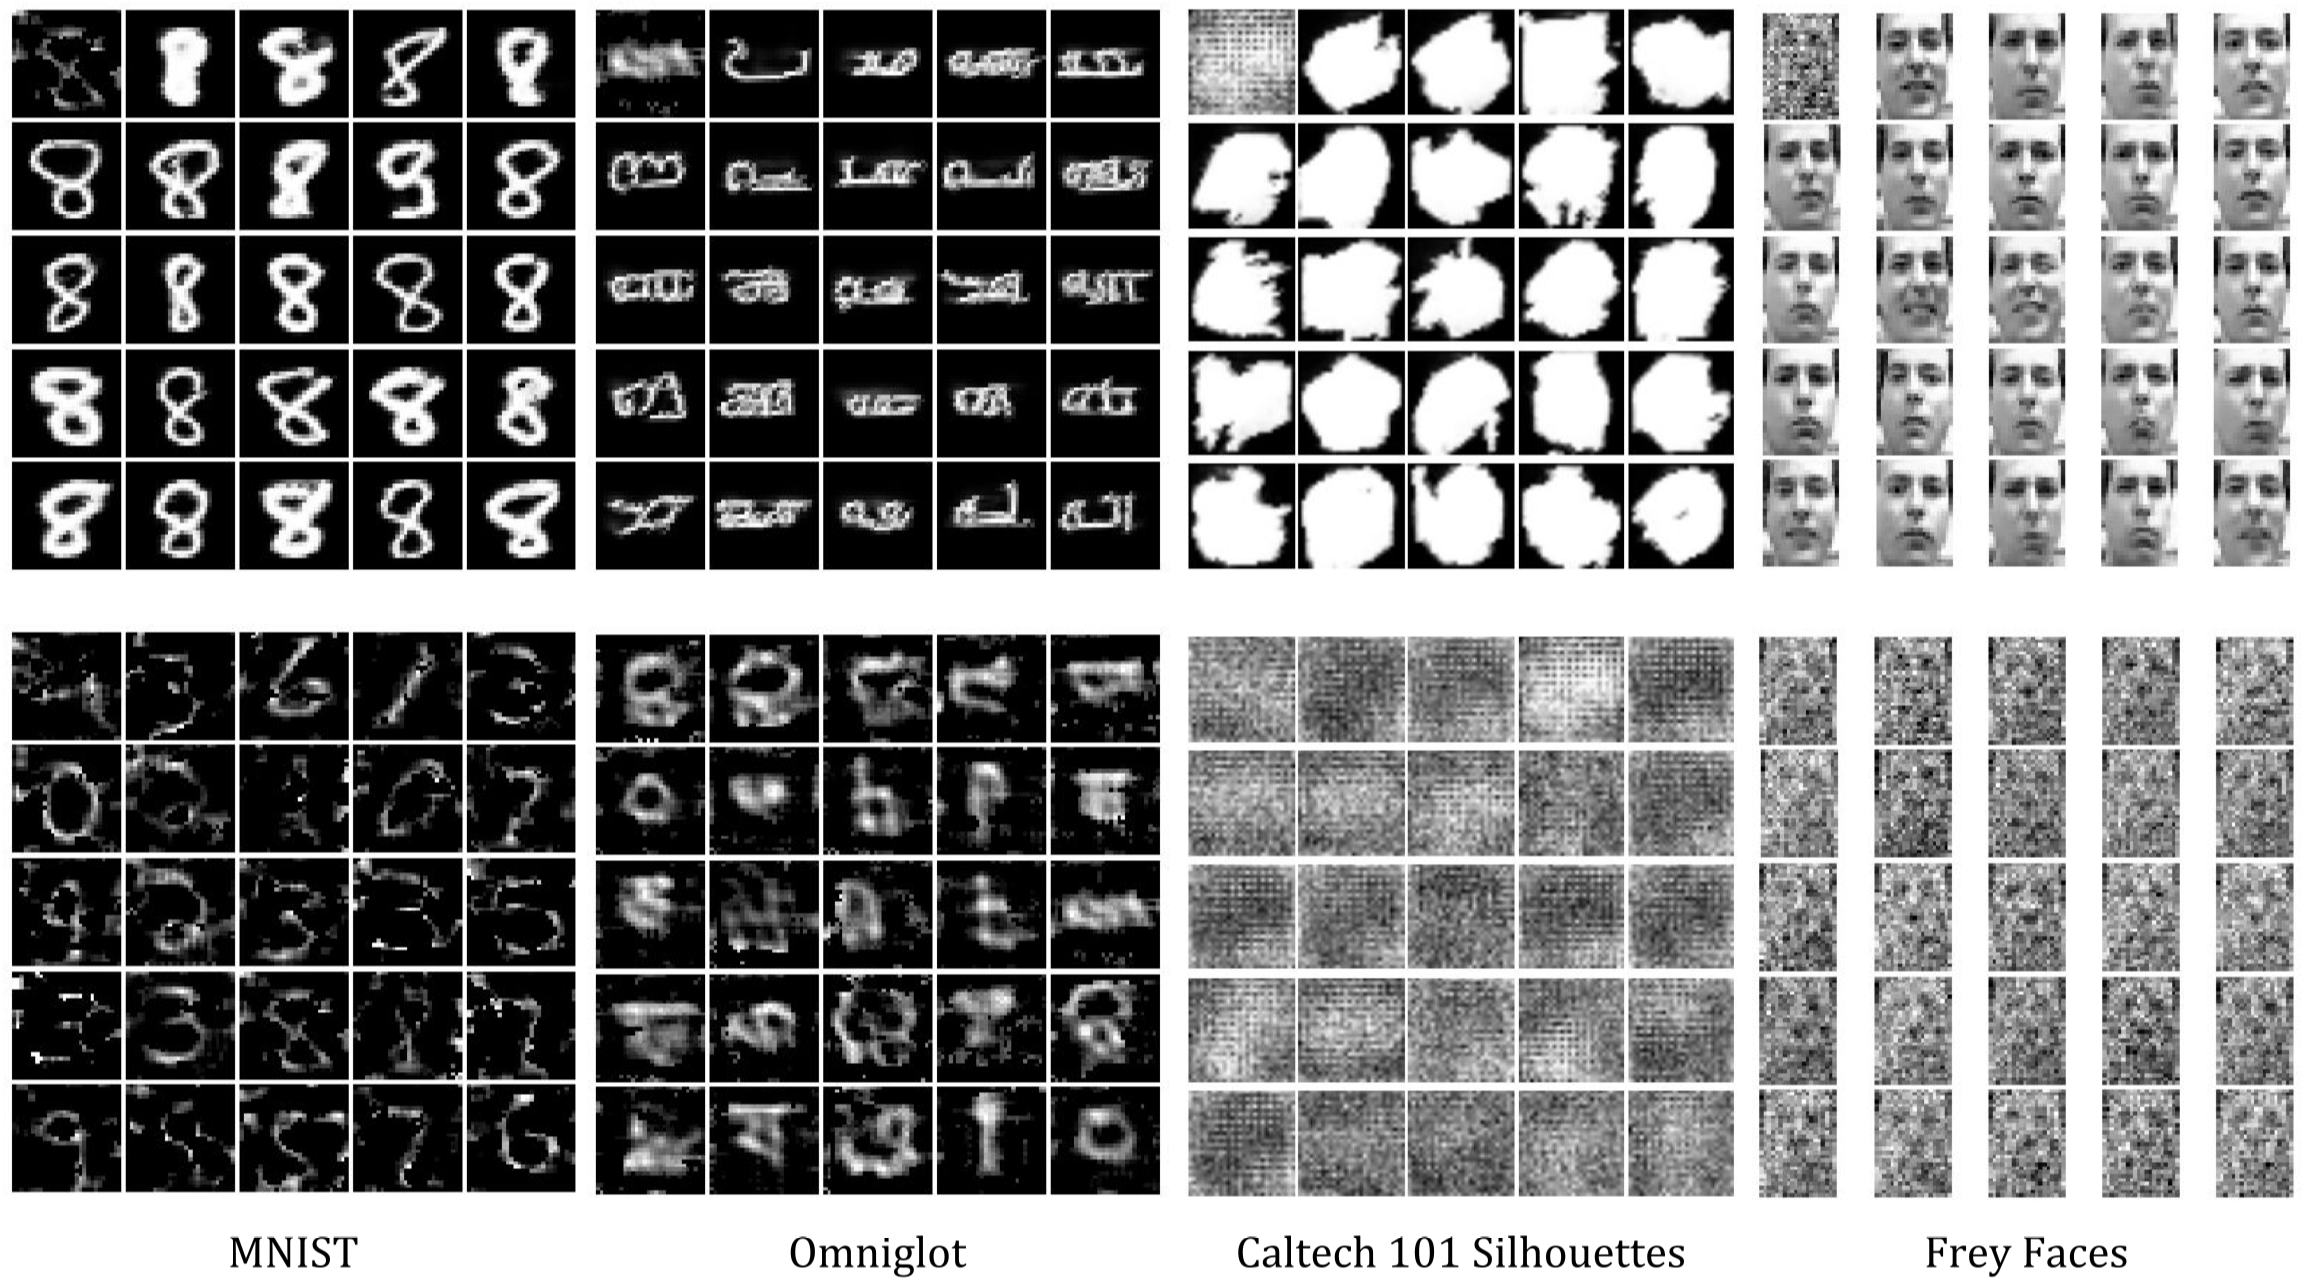
\includegraphics[width=1.0\linewidth]{figs/VampPrior_4.png}
	\end{figure}
	\myfootnotewithlink{https://arxiv.org/abs/1705.07120}{Tomczak J. M., Welling M. VAE with a VampPrior, 2017}
\end{frame}
%=======
\begin{frame}{Flow prior in VAE}
	
	\begin{block}{ELBO revisiting}
		\vspace{-0.3cm}
		{\footnotesize
			\[
			\mathcal{L}(q, \btheta) = \underbrace{\frac{1}{n} \sum_{i=1}^n \mathbb{E}_{q(\bz_i | \bx_i)} \log p(\bx_i | \bz_i, \btheta)}_{\text{Reconstruction loss}} - \underbrace{\left(\log n - \mathbb{E}_{q(\bz)} \mathbb{H} \left[ q(i | \bz) \right] \right)\vphantom{\sum_{i=1}}}_{0 \leq \text{Mutual info} \leq \log N } - \underbrace{KL(q(\bz) || p(\bz))\vphantom{\sum_{i=1}}}_{\text{Marginal KL}}
			\]}
	\end{block}
	\vspace{-0.5cm}
	\begin{block}{VampPrior}
		\vspace{-0.5cm}
		\[
			p(\bz | \blambda) = \frac{1}{K} \sum_{k=1}^K q(\bz | \bu_k),
		\]
	where $\bu_1, \dots \bu_K$ is trainable preudo-inputs.
	\end{block}
	\begin{block}{Autoregressive flow prior}
		\vspace{-0.5cm}
		\[
			\log p(\bz | \blambda) = \log p(\bepsilon) + \log \det \left | \frac{d \bepsilon}{d\bz}\right|
		\]
		\[
			\bz = g(\bepsilon, \blambda) = f^{-1}(\bepsilon, \blambda) 
		\]
	\end{block}
	\myfootnotewithlink{https://arxiv.org/abs/1611.02731}{Chen X. et al. Variational Lossy Autoencoder, 2016}
\end{frame}
%=======
\begin{frame}{Variational Lossy AutoEncoder, 2016}
	\begin{block}{Theorem}
	VAE with the AF prior for latent code $\bz$ is equivalent to using the IAF posterior for latent code $\bepsilon$.
	\end{block}
	\begin{block}{Proof}
	\vspace{-0.5cm}
	{\footnotesize
	\begin{align*}
	\mathcal{L}(q, \btheta) &= \mathbb{E}_{q(\bz | \bx)} \left[ \log p(\bx | \bz, \btheta) +  \log p(\bz, \blambda) - q(\bz | \bx) \right] \\
	&= \mathbb{E}_{\bz \sim q(\bz | \bx)} \Bigl[ \log p(\bx | \bz, \btheta) + \underbrace{ \Bigl( \log p(f(\bz, \blambda)) + \log \left| \det \frac{\partial f(\bz, \blambda)}{\partial \bz} \right| \Bigr) }_{\text{AF prior}} - q(\bz | \bx) \Bigr] \\
	&= \mathbb{E}_{\bz \sim q(\bz | \bx)} \Bigl[ \log p(\bx | \bz, \btheta) +  \log p(f(\bz, \blambda)) - \underbrace{ \Bigl( q(\bz | \bx) - \log \left| \det \frac{\partial f(\bz, \blambda)}{\partial \bz} \right| \Bigr) }_{\text{IAF posterior}} \Bigr]
	\end{align*}
	}
	\end{block}
	\vspace{-0.5cm}
	\begin{block}{Flows in VAE}
		\vspace{-0.3cm}
		{\footnotesize
		\[
			\mathcal{L} (\bphi, \btheta) 
			= \mathbb{E}_{q(\bz_0 | \bx, \bphi)} \bigg[\log p(\bx, \bz_K | \btheta) -  \log q(\bz_0 | \bx, \bphi ) +   \log \left| \det \left( \frac{\partial g(\bz_0, \bphi_*)}{\partial \bz_0} \right) \right| \bigg].
		\]
		}
	\end{block}
	\myfootnotewithlink{https://arxiv.org/abs/1611.02731}{Chen X. et al. Variational Lossy Autoencoder, 2016}
\end{frame}
%=======
\begin{frame}{Variational Lossy AutoEncoder, 2016}
	\begin{block}{Autoregressive flow prior}
		{\footnotesize
		\begin{align*}
			\mathcal{L}(q, \btheta) &= \mathbb{E}_{\bz \sim q(\bz | \bx)} \Bigl[ \log p(\bx | \bz, \btheta) + \underbrace{ \Bigl( \log p(f(\bz, \blambda)) + \log \left| \det \frac{\partial f(\bz, \blambda)}{\partial \bz} \right| \Bigr) }_{\text{AF prior}} - q(\bz | \bx) \Bigr] \\
			&= \mathbb{E}_{\bz \sim q(\bz | \bx)} \Bigl[ \log p(\bx | \bz, \btheta) +  \log p(f(\bz, \blambda)) - \underbrace{ \Bigl( q(\bz | \bx) - \log \left| \det \frac{\partial f(\bz, \blambda)}{\partial \bz} \right| \Bigr) }_{\text{IAF posterior}} \Bigr]
		\end{align*}
		}
	\end{block}
	\begin{itemize}
		\item IAF posterior decoder path: $p(\bx|\bz, \btheta)$, $\bz \sim p(\bz)$.
		\item AF prior decoder path: $p(\bx|\bz, \btheta)$, $\bz = g(\bepsilon, \blambda)$, $\bepsilon \sim p(\bepsilon)$. 
	\end{itemize}
	The AF prior and the IAF posterior have the same computation cost, so using the AF prior makes the model more expressive at no training time cost.

	\myfootnotewithlink{https://arxiv.org/abs/1611.02731}{Chen X. et al. Variational Lossy Autoencoder, 2016}
\end{frame}
%=======
\begin{frame}{Summary}
	\begin{itemize}
		\item Uniform dequantization is the simplest form of dequantization. Variational dequantization is a more natural type that was proposed in Flow++ model.
		\vfill
		\item The importance sampling could get the tighter lower bound to the likelihood.
		\vfill
		\item The ELBO surgery reveals insights about a prior distribution in VAE. The optimal prior is the aggregated posterior.
		\vfill
		\item VampPrior proposes to use a variational mixture of posteriors as the prior to approximate the aggregated posterior.
		\vfill
		\item The autoregressive flows could be used as the prior. This is equivalent to the use of the IAF posterior. 
	\end{itemize}
\end{frame}

\end{document} 